%%%%%%%%%%%%%%%%%%%%%%%%%%%%%%%%%%%%%%%%%%%%%%%%%%%%%%%%%%%%%%%%%%%%%%%%%%%%%%%%
\section{Radiation Transport}
\label{sec:bg:rt}
%%%%%%%%%%%%%%%%%%%%%%%%%%%%%%%%%%%%%%%%%%%%%%%%%%%%%%%%%%%%%%%%%%%%%%%%%%%%%%%%

The most fundamental equation in radiation transport is the transport equation, which is sometimes referred to as the neutron transport equation or the Boltzmann equation.
The transport equation can be used to solve for the particle flux, which is a measure of how many particles are passing through an area per unit time.
Calculating the flux at some location or locations is almost always necessary when performing radiation transport calculations.

This section describes the transport equation, the concept of adjoint transport, and two classes of methods used to solve the transport equation: deterministic methods and the Monte Carlo method.

% Much of the information in sections \ref{sec:bg:rt:te} and \ref{sec:bg:rt:at} is paraphrased from the textbook by Lewis \& Miller \cite{lewis_miller}.
Much of the information in this section is paraphrased from the textbook by Lewis \& Miller \cite{lewis_miller}.

%===============================================================================
\subsection{Transport Equation}
\label{sec:bg:rt:te}
%===============================================================================

%-------------------------------------------------------------------------------
\subsubsection{Particle Distributions}
\label{sec:bg:rt:te:pd}
%-------------------------------------------------------------------------------

In general, there are seven independent variables that are required to fully describe the distribution of particles: three coordinates specifying position ($\vec{r}$), two angles specifying the particle's direction of travel ($\hat{\Omega}$), the particle's energy ($E$), and time ($t$).
These seven variables describe the \textit{phase space} of a problem.

In steady-state problems, there is no dependence on time, and thus there are only six independent variables (three for position, two for angle, and one for energy.) The remainder of this work will only consider time-independent problems, so the dependence on time will be neglected.

The most fundamental dependent variable in transport theory is the \textit{particle density distribution}.
The particle density distribution $N\left(\vec{r},\hat{\Omega},E\right)dEd\hat{\Omega}dV$ is defined as the number of particles in a volume element $dV$ about $\vec{r}$ traveling in the cone of directions $d\hat{\Omega}$ about $\hat{\Omega}$ with energies between $E$ and $E + dE$.

The particle density distribution is rarely directly considered in transport calculations, however.
The most common quantity considered is the \textit{angular flux}:
\begin{equation}\label{eq:bg:rt:angular-flux}
  \psi\left(\vec{r},\hat{\Omega},E\right) \equiv vN\left(\vec{r},\hat{\Omega},E\right)
\end{equation}
where $v$ is the particle speed.

It is sometimes useful to consider the flux independent of angle.
In these cases, the \textit{scalar flux} may be considered:
\begin{equation}\label{eq:bg:rt:scalar-flux}
  \phi\left(\vec{r},E\right) \equiv \int_{4\pi}\psi\left(\vec{r},\hat{\Omega},E\right)d\hat{\Omega}.
\end{equation}

The \textit{current vector}, which is a measure of the directionality of particles, is defined as
\begin{equation}\label{eq:bg:rt:current-vector}
  \vec{J}\left(\vec{r},E\right) \equiv \int_{4\pi}\psi\left(\vec{r},\hat{\Omega},E\right)\hat{\Omega} d\hat{\Omega}.
\end{equation}

The \textit{reaction rate} for reactions of type $x$ is
\begin{equation}\label{eq:bg:rt:rxn-rate-angular}
  R = \int_V\int_{4\pi}\int_0^\infty\sigma_x\left(\vec{r},\hat{\Omega},E\right)\psi\left(\vec{r},\hat{\Omega},E\right)dEd\hat{\Omega}dV
\end{equation}
where $\sigma_x$ is the cross section for reaction $x$.
Cross sections are almost always independent of the particle direction, so the reaction rate equation can be simplified as
\begin{equation}\label{eq:bg:rt:rxn-rate-scalar}
  R = \int_V\int_0^\infty\sigma_x\left(\vec{r},E\right)\phi\left(\vec{r},E\right)dEdV.
\end{equation}

If $\sigma_x$ refers to the total cross section $\sigma_t$, then the reaction rate is referred to as the \textit{collision density}.

%-------------------------------------------------------------------------------
\subsubsection{Transport Equation with General Source}
\label{sec:bg:rt:te:te}
%-------------------------------------------------------------------------------

The transport equation is a balance between all possible mechanisms for the number of particles in $dEd\hat{\Omega}dV$ to change.
There are three such mechanisms:
\begin{enumerate}
  \item net streaming out of $dV$, given by the streaming term $\hat{\Omega}\cdot\vec{\nabla}\psi\left(\vec{r},\hat{\Omega},E\right)$,
  \item collisions in $dV$ that result in particle absorption or scattering out of $dEdV$, given by the collision term $\sigma_t\left(\vec{r},E\right)\psi\left(\vec{r},\hat{\Omega},E\right)$, and
  \item emission of particles in $dV$ (includes external sources, scattering, and fission), given by a general source term $q\left(\vec{r},\hat{\Omega},E\right)$.
\end{enumerate}

The time-independent transport equation is a balance between these three processes, and it is given by
\begin{equation}\label{eq:bg:rt:transport-totsrc}
  \hat{\Omega}\cdot\vec{\nabla}\psi\left(\vec{r},\hat{\Omega},E\right) +
  \sigma_t\left(\vec{r},E\right)\psi\left(\vec{r},\hat{\Omega},E\right) =
  q\left(\vec{r},\hat{\Omega},E\right).
\end{equation}

%-------------------------------------------------------------------------------
\subsubsection{Source Terms}
\label{sec:bg:rt:te:st}
%-------------------------------------------------------------------------------

The source term $q\left(\vec{r},\hat{\Omega},E\right)$ includes contributions from three sources: external sources, scattering, and fission.
It can be represented as a sum of these three contributions:
\begin{equation}\label{eq:bg:rt:source}
  q = q_{ex} + q_s + q_f.
\end{equation}

External sources are known distributions of source particles that are entirely independent of the flux.
External sources are represented as a known distribution $q_{ex}\left(\vec{r},\hat{\Omega},E\right)$.

Scattering sources are the result of particles scattering from one angle and energy to another.
Particles at the original angle and energy are removed from the system while particles at the new angle and energy are born.
The source due to scattering is given by the scattering term:
\begin{equation}\label{eq:bg:rt:scattering-term}
  q_s\left(\vec{r},\hat{\Omega},E\right) \equiv
  \int_{4\pi}\int_0^\infty\sigma_s\left(\vec{r},\hat{\Omega}^\prime\rightarrow\hat{\Omega},E^\prime\rightarrow E\right)\psi\left(\vec{r},\hat{\Omega}^\prime,E^\prime\right)dE^\prime d\hat{\Omega}^\prime
\end{equation}
where the scattering cross section $\sigma_s\left(\vec{r},\hat{\Omega}^\prime\rightarrow\hat{\Omega},E^\prime\rightarrow E\right)$ is the cross section for particles to scatter from $\hat{\Omega}^\prime$ into $\hat{\Omega}$ and $E^\prime$ into $E$.

Fission sources only occur if a multiplying medium exists in the system.
Fission sources will not be considered in this work.

Separating the total source term in the time-independent transport equation into its external and scattering components yields
\begin{multline}\label{eq:bg:rt:transport}
  \hat{\Omega}\cdot\vec{\nabla}\psi\left(\vec{r},\hat{\Omega},E\right) +
  \sigma_t\left(\vec{r},E\right)\psi\left(\vec{r},\hat{\Omega},E\right) = \\
  \int_{4\pi}\int_0^\infty\sigma_s\left(\vec{r},\hat{\Omega}^\prime\rightarrow\hat{\Omega},E^\prime\rightarrow E\right)\psi\left(\vec{r},\hat{\Omega}^\prime,E^\prime\right)dE^\prime d\hat{\Omega}^\prime +
  q\left(\vec{r},\hat{\Omega},E\right).
\end{multline}

%-------------------------------------------------------------------------------
\subsubsection{Operator Notation}
\label{sec:bg:rt:te:on}
%-------------------------------------------------------------------------------

It is often useful to write the transport equation in operator notation.
In this case, the time-independent \textit{transport operator} $H$ operates on the angular flux $\psi$ and is given by
\begin{multline}\label{eq:bg:rt:transport-operator}
  H\psi \equiv
  \hat{\Omega}\cdot\vec{\nabla}\psi\left(\vec{r},\hat{\Omega},E\right) +
  \sigma_t\left(\vec{r},E\right)\psi\left(\vec{r},\hat{\Omega},E\right) - \\
  \int_{4\pi}\int_0^\infty\sigma_s\left(\vec{r},\hat{\Omega}^\prime\rightarrow\hat{\Omega},E^\prime\rightarrow E\right)\psi\left(\vec{r},\hat{\Omega}^\prime,E^\prime\right)dE^\prime d\hat{\Omega}^\prime.
\end{multline}
The transport equation in operator notation is then simply
\begin{equation}\label{eq:bg:rt:transport-opnot}
  H\psi = q.
\end{equation}

%===============================================================================
\subsection{Adjoint Transport}
\label{sec:bg:rt:at}
%===============================================================================

Given an operator $H$ and the functions $\zeta$ and $\zeta^+$, the adjoint operator $H^+$ is defined by the \textit{adjoint identity}
\begin{equation}\label{eq:bg:rt:adjoint-identity}
  \left<\zeta^+,H\zeta\right> =
  \left<\zeta,H^+\zeta^+\right>,
\end{equation}
where $\left<\right>$ denotes integration over all independent variables.

It is often useful to consider adjoint transport, as distinct from forward (regular) transport.
An adjoint transport operator $H^+$ exists which satisfies the adjoint identity and operates on the \textit{adjoint flux} $\psi^+$.
The adjoint transport equation in operator notation is
\begin{equation}\label{eq:bg:rt:adjtransport-opnot}
  H^+\psi^+ = q^+,
\end{equation}
where $q^+$ is the adjoint source.
It is most useful to define the adjoint source as some detector response in the forward system.

Adjoint transport can be thought of as running in reverse when compared to forward transport.
In a system with a source and a detector, particles stream outward from the source and a response is calculated at the detector.
Adjoint particles, however, stream outward from the detector and a response is calculated at the source.
Adjoint particles also undergo scattering in reverse, gaining energy through scattering instead of losing energy.

There is a physical interpretation of the adjoint flux: the adjoint flux at a point is equal to the \textit{importance} of particles emitted at that point to the detector response.
In other words, the adjoint flux at some location $\vec{r}_0, \hat{\Omega}_0, E_0$ indicates how much a source at that location would contribute to the detector response.

The time-independent adjoint operator $H^+$ operates on the adjoint angular flux $\psi^+$ and is given by
\begin{multline}\label{eq:bg:rt:transport-operator}
  H^+\psi^+ \equiv
  -\hat{\Omega}\cdot\vec{\nabla}\psi^+\left(\vec{r},\hat{\Omega},E\right) +
  \sigma_t\left(\vec{r},E\right)\psi^+\left(\vec{r},\hat{\Omega},E\right) - \\
  \int_{4\pi}\int_0^\infty\sigma_s\left(\vec{r},\hat{\Omega}\rightarrow\hat{\Omega}^\prime,E\rightarrow E^\prime\right)\psi^+\left(\vec{r},\hat{\Omega}^\prime,E^\prime\right)dE^\prime d\hat{\Omega}^\prime.
\end{multline}

After expanding the adjoint transport operator, the adjoint transport equation is given by
\begin{multline}\label{eq:bg:rt:adjoint-transport}
  -\hat{\Omega}\cdot\vec{\nabla}\psi^+\left(\vec{r},\hat{\Omega},E\right) +
  \sigma_t\left(\vec{r},E\right)\psi^+\left(\vec{r},\hat{\Omega},E\right) = \\
  \int_{4\pi}\int_0^\infty\sigma_s\left(\vec{r},\hat{\Omega}\rightarrow\hat{\Omega}^\prime,E\rightarrow E^\prime\right)\psi^+\left(\vec{r},\hat{\Omega}^\prime,E^\prime\right)dE^\prime d\hat{\Omega}^\prime +
  q^+\left(\vec{r},\hat{\Omega},E\right).
\end{multline}

The detector response $R$ can be calculated in two ways:
\begin{equation}\label{eq:bg:rt:detector-response}
  R = \left<\psi,q^+\right>
    = \left<\psi^+,q\right>.
\end{equation}

%===============================================================================
\subsubsection{Adjoint and Combined Particle Distributions}
\label{sec:bg:rt:at:apd}
%===============================================================================

Several important particle distributions that exist in forward transport also exist in adjoint transport.
The adjoint scalar flux is defined as
\begin{equation}\label{eq:bg:rt:scalar-flux}
  \phi^+\left(\vec{r},E\right) \equiv
  \int_{4\pi}\psi^+\left(\vec{r},\hat{\Omega},E\right)d\hat{\Omega}.
\end{equation}
The adjoint current vector is defined as
\begin{equation}\label{eq:bg:rt:current-vector}
  \vec{J}^+\left(\vec{r},E\right) \equiv
  \int_{4\pi}\psi^+\left(\vec{r},\hat{\Omega},E\right)\hat{\Omega} d\hat{\Omega}.
\end{equation}

There are also some distributions that combine both the forward and adjoint flux.
The angular \textit{contributon flux} is defined as the product of the forward and adjoint angular fluxes:
\begin{equation}\label{eq:bg:rt:angular-contributon}
  \psi_{contrib}\left(\vec{r},\hat{\Omega},E\right) \equiv
  \psi\left(\vec{r},\hat{\Omega},E\right)\psi^+\left(\vec{r},-\hat{\Omega},E\right).
\end{equation}
The scalar contributon flux is obtained by integrating the angular contribution flux over angle:
\begin{equation}\label{eq:bg:rt:angular-contributon}
  \phi_{contrib}\left(\vec{r},E\right) \equiv
  \int_{4\pi}\psi\left(\vec{r},\hat{\Omega},E\right)\psi^+\left(\vec{r},-\hat{\Omega},E\right)d\hat{\Omega}.
\end{equation}
Note that this is not the same quantity as the product of the forward and adjoint scalar fluxes. It is important to integrate over energy after multiplying the forward and angular fluxes, not before.

%===============================================================================
\subsection{Deterministic Methods}
\label{sec:bg:rt:determ}
%===============================================================================

Deterministic methods aim to solve the transport equation directly, and they generally produce detailed solutions throughout the entire phase space (space, angle, and energy) of a problem.

The most common types of deterministic methods used to solve the transport equation are the \textit{discrete ordinates methods}.
In three spatial dimensions, discrete ordinates methods are known as S\textsubscript{N} methods.
In the discrete ordinates method, phase space is divided into discrete sections, and particles can be thought of as moving from section to section.
Physical space is divided into boxes, angle space is divided into discrete angles, and energy space is divided into energy bins.
Figure \ref{fig:bg:discrete-ordinates} shows a visualization of the type of angle discretization present in S\textsubscript{N} methods.

\begin{figure}[h!]
  \centering
  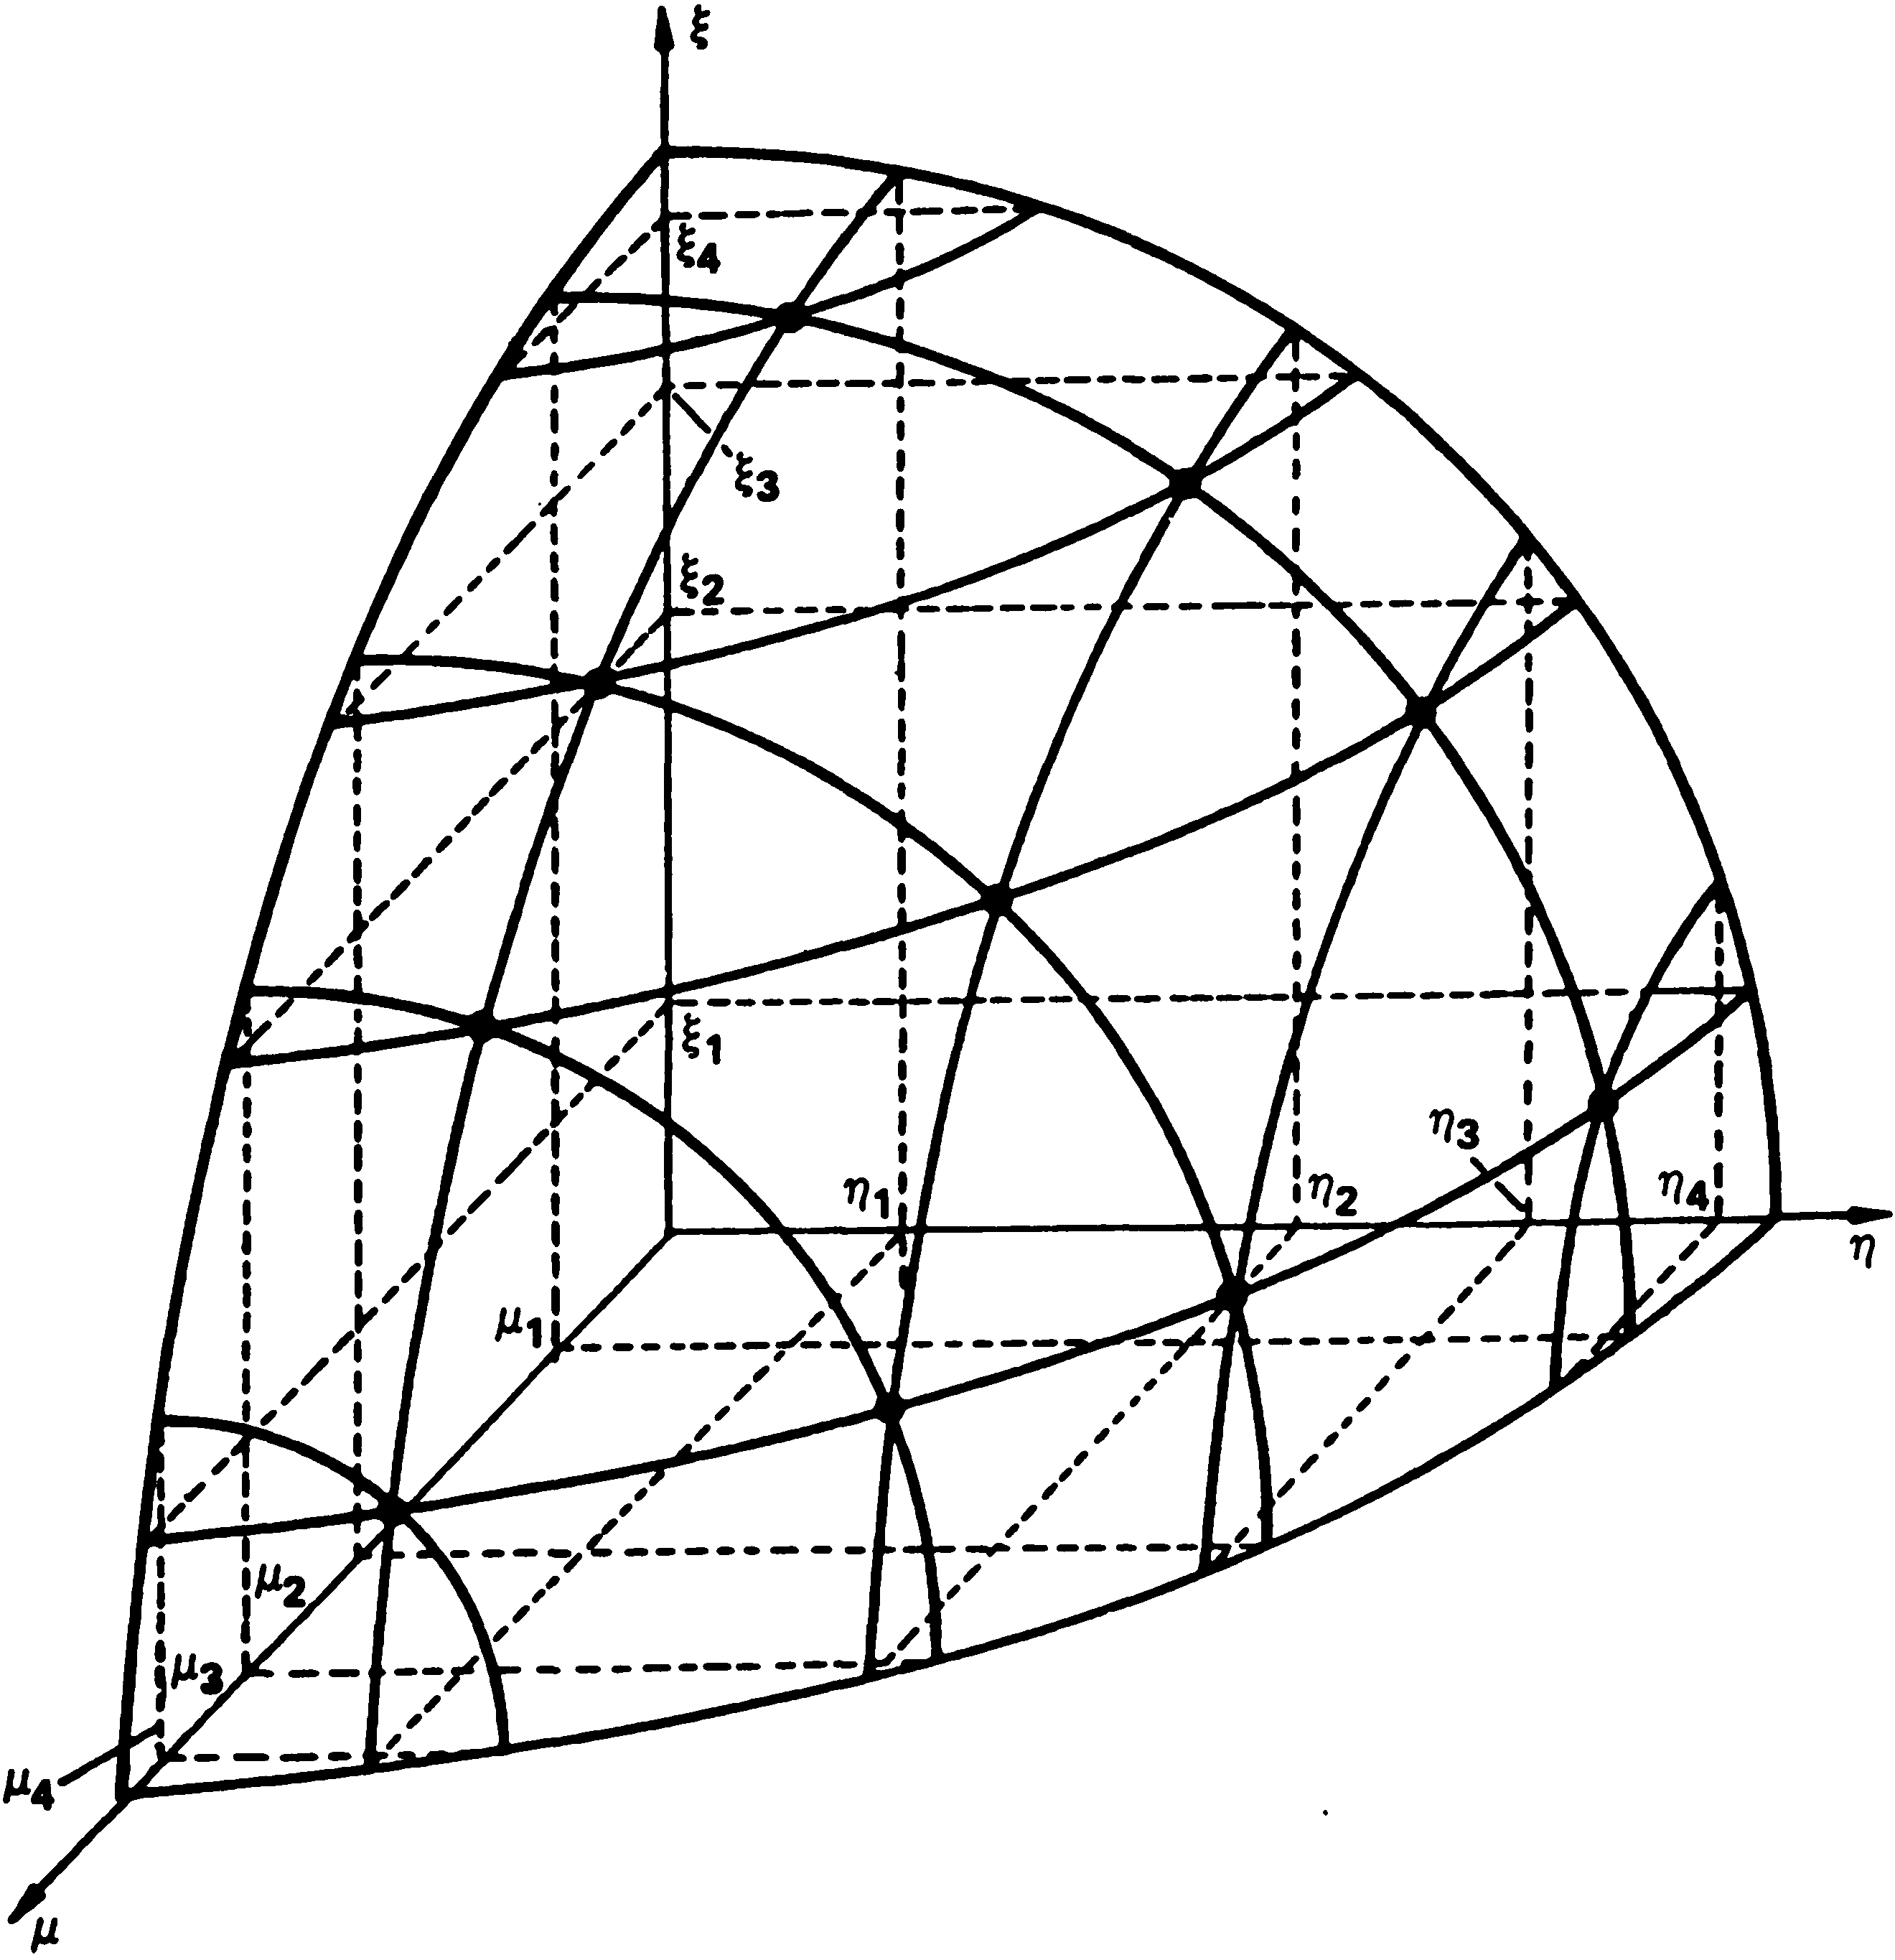
\includegraphics[width=0.7\textwidth]{content/background/discrete_ordinates.png}
  \caption{Visualization of the S\textsubscript{8} discrete ordinates set (taken from \cite{lewis_miller}.)}
  \label{fig:bg:discrete-ordinates}
\end{figure}

This discretization introduces uncertainties in the results.
Real-world geometries cannot be perfectly divided into boxes, real-world particles can move in any direction, and real-world cross sections are continuous in energy.
It is possible to increase the fidelity of a model by decreasing the size of the boxes, but at the cost of an increased amount of computation.
Additionally, discrete ordinates methods can sometimes produce non-physical results such as ray effects (caused by the angle discretization) and negative fluxes (caused by certain types of spatial discretization).

For all of these reasons, deterministic methods are rarely suitable by themselves for use in the analysis of complex nuclear systems.

Deterministic methods are not entirely without use though.
For example, in deep penetration problems (with which Monte Carlo methods have considerably difficulty,) deterministic methods can be used to solve the forward and adjoint transport equations and generate weight window parameters for use in Monte Carlo radiation transport (i.e. the FW-CADIS method \cite{fwcadis} in the ADVANTG \cite{advantg} software package.)
In these cases, it is not necessary that the deterministic solver produce a perfectly accurate solution because the end results are still derived from the Monte Carlo simulation; an approximate solution is sufficient.

%-------------------------------------------------------------------------------
\subsubsection{Denovo}
\label{sec:bg:rt:determ:denovo}
%-------------------------------------------------------------------------------

Denovo \cite{denovo} is a powerful block-parallel S\textsubscript{N} code developed at Oak Ridge National Laboratory.
It uses the multigroup energy and anisotropic P\textsubscript{n} approximations, and it can solve both the forward and adjoint transport equations.
It has several spatial discretization algorithms and angle quadrature sets and has numerous additional options and features that allow users to control problem parameters.
Denovo has been used to solve problems with over a billion voxels.

%===============================================================================
\subsection{Monte Carlo Method}
\label{sec:bg:rt:mc}
%===============================================================================

The Monte Carlo method takes a fundamentally different approach to solving the transport equation than deterministic methods.
In the Monte Carlo method, individual particles are simulated, and results are inferred from the average particle behavior.
Results are only obtained for specific quantities, called tallies, that are requested by the user.
Phase space is not discretized, so accurate results can be obtained for highly complicated problems.

Monte Carlo codes use random numbers to sample probability distributions that specify the likelihood that a particle will undergo various physical processes.
Random numbers are used to sample the distance a particle travels before undergoing an interaction, called the path length, and they are also used to randomly sample the type of interaction that occurs, examples of which are scattering, absorption, and fission.
Secondary particles, such as a photon being created due to a neutron inelastic scattering event, are also tracked.
Figure \ref{fig:bg:monte-carlo} shows an example of a random particle history simulated by a Monte Carlo code. 

\begin{figure}[h!]
  \centering
  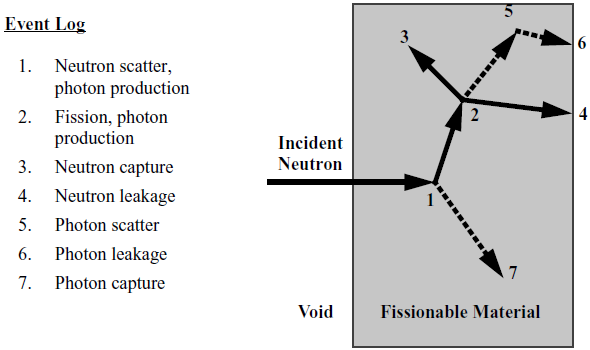
\includegraphics[width=1.0\textwidth]{content/background/monte_carlo.png}
  \caption{Visualization of a random history of a neutron entering a slab of fissionable material (taken from \cite{mcnp5_vol1}.)}
  \label{fig:bg:monte-carlo}
\end{figure}

Since Monte Carlo codes simulate particles randomly and infer results based on average particle behavior, every result obtained from Monte Carlo codes have an associated uncertainty.
The more particles simulated, the lower the uncertainty.
For highly complex problems, the number of particles that must be simulated in order to obtain reliable results is on the order of billions.
This means that Monte Carlo simulations are generally much more computationally expensive than determinstic simulations.

%-------------------------------------------------------------------------------
\subsubsection{MCNP}
\label{sec:bg:rt:mc:mcnp}
%-------------------------------------------------------------------------------

The \ac{mcnp} transport code \cite{mcnp620} is a powerful and widely-used parallel Monte Carlo code developed at Los Alamos National Laboratory.

MCNP allows for arbitrary geometry representations using a text-based \ac{csg} language.
It operates in continuous energy space and is designed to track particles over a wide range of energies.
It can track many different types of neutral and charged particles, with neutrons, photons, and electrons being the most common.
It is used for nuclear analysis and design in a wide range of applications, including radiation protection, shielding, radiography, medical physics, criticality safety, detectors, accelerators, fission reactors, and fusion reactors.

Users must create an input file to run MCNP.
The input file contains the problem geometry, material assignments and definitions, source definition, and tally definitions, and may also contain numerous other parameters which alter the code's operation in some way.

%-------------------------------------------------------------------------------
\subsection{ADVANTG}
\label{sec:bg:rt:advantg}
%-------------------------------------------------------------------------------

The \ac{advantg} \cite{advantg} software developed at Oak Ridge National Laboratory provides easy access to the Denovo discrete ordinates solver.
The main purpose of ADVANTG is to generate variance reduction parameters for use in Monte Carlo simulations, but it can also be used simply to drive Denovo calculations without calculating any variance reduction parameters.

Here are the main steps involved when using ADVANTG to drive a Denovo calculation:
\begin{itemize}
  \item Generate an MCNP ``runtpe'' file from the user-supplied MCNP input file.
  \item Extract information about the geometry, materials, sources, and tallies from the runtpe file.
  \item Mix the multigroup cross sections.
  \item Map the materials, sources, and tallies onto the spatial grid and energy bins.
  \item Execute Denovo (forward transport, adjoint transport, or both.)
  \item Write output to file.
\end{itemize}

ADVANTG contains a number of multigroup cross section libraries for neutrons and gammas.
These libraries contain data for up to 393 different isotopes, and are based on the ENDF/B-VII.0 \cite{endfb7.0} evaluated nuclear data library.

Materials are mapped onto the spatial mesh via ray tracing.
Track-length tallies are used to calculate the volume fraction of each material in each voxel.
If two voxels have the material volume fractions that are not exactly the same but are similar to within a user-specified tolerance, then ADVANTG will treat them as the same material to conserve memory.

ADVANTG can handle both point sources and volume sources, and it calculates the multigroup energy spectrum for each source.
Point sources often cause unwanted ray effects, so first-collided sources based on the uncollided flux distribution are calculated by default for point sources.
In this case, the total flux is then the sum of the uncollided flux and the result of the discrete ordinates calculation for the first-collided source.
This feature is also available for volume sources, but it is not enabled by default.

Point sources are mapped onto the spatial mesh exactly.
Volume sources are mapped onto the spatial mesh stochastically by sampling source particles and tallying the weight of particles born in each voxel.

Surface, cell, and mesh tallies are mapped onto the spatial mesh via the same process as the material mapping. A multigroup energy spectrum is calculated for each tally which is based on MCNP dose responses or tally multipliers.

The main outputs of ADVANTG when it it is used to drive deterministic calculations are Silo files \cite{silo}.
These files contain information about the spatial grid, mixed materials, sources, and tallies mapped onto the grid, the scalar forward and adjoint fluxes, and the contributon flux.
The data contained in the Silo files can be visualized easily with the VisIT software \cite{visit}.

Denovo calculates the full forward and angular angular fluxes as part of its calculation process.
However, there are no documented user options which allow users to access this angular flux data.
Luckily, ADVANTG does contain an undocumented feature which allows for the full angular flux data to be written to an HDF5 file \cite{hdf5}.
